\documentclass[11pt,a4paper]{article}
\usepackage[hyperref]{acl2020}
\usepackage{times}
\usepackage{amsfonts}
\usepackage{amsmath}
\usepackage{latexsym}
\usepackage{graphicx}
\renewcommand{\UrlFont}{\ttfamily\small}

\usepackage{microtype}

\aclfinalcopy

\newcommand\BibTeX{B\textsc{ib}\TeX}

\title{Tutela: An Anonymity Tool for Ethereum and Tornado Cash}

\author{
  \small{Mike Wu, Will McTighe, Kaili Wang}\\
  \small{Stanford University} \\ \And
  \small{Nick Bax} \\
  \small{Convex Research} \\ \And
  \small{Istv\'{a}n A. Seres} \\
  \small{E\"{o}tv\"{o}s Lor\'{a}nd University} \\ \AND
  \small{Frederico Carrone, Tomas De Mattey, Manuel Puebla, Herman O. Demaestri, Mariano Nicolini, Pedro Fontana} \\
  \small{LambdaClass} \\}
\date{}

\begin{document}
\maketitle
\begin{abstract}
A common misconception among blockchain users is that decentralization guarantees privacy. The reality is almost the opposite as every transaction one makes, being recorded on a public ledger, reveals information about one's identity.
Mixers, such as Tornado Cash, were developed to preserve privacy through ``mixing'' transactions in an anonymity pool, such that it is impossible to identify who withdrew tokens from the pool. Unfortunately, it is still possible to reveal information about those in the anonymity pool if users are not careful.
We introduce Tutela, an application built on expert heuristics to report the true anonymity of an Ethereum address.
In particular, Tutela has two functionalities: first, it clusters together Ethereum addresses based on interaction history such that for an Ethereum address, we can identify other addresses likely owned by the same entity; second, Tutela computes the true size of the anonymity pool of Tornado Cash mixing, taking into account compromised addresses that reveal identity information. A public implementation of Tutela can be found at \url{https://github.com/TutelaLabs/tutela-app}.
\end{abstract}

\section{Introduction}

On any modern blockchain, the cost of creating a new wallet, being virtually zero, enables the same entity to manage several pseudonymous addresses. The decentralization underpinning blockchains like Bitcoin \citep{nakamoto2008bitcoin} and Ethereum \citep{buterin2013ethereum}, breeds a sense of privacy. This often leads to misuse \citep{christin2013traveling}, such as money laundering through a large number of addresses \citep{moser2013inquiry}, or unfair voting power distributed among multiple addresses owned by the same user. Thus, it is of interest in many investigations to identify addresses linked to the same entity. This is predominantly done through heuristics. Every transaction an address makes on the blockchain, being a public ledger, reveals information about the underlying entity. As such, with graph analysis tools, one can cluster addresses together that with reasonable confidence, possess the same owner.

Such anonymity tools have been widely explored for Bitcoin \cite{haslhofer2016bitcoin,kappos2018empirical}, leveraging heuristics targeting the unspent transaction (UTXO) model. However, this has limited application to more recent blockchain implementations like Ethereum, that forgo the UTXO model for a smart contract model.
Ethereum, in particular, has an account-based protocol that implicitly encourages an entity to reuse a handful of addresses.
As such, this poses greater challenges to user privacy than UTXO-based blockchains.

In response to this shortcoming, several coin mixing protocols have been proposed like M\"{o}bius \citep{meiklejohn2018mobius}, MixEth \citep{seres2019mixeth}, and Tornado Cash \citep{pertsev2019tornado} to obfuscate transaction tracing, the final of which is deployed in practice.
 % As this has limited application to more recent blockchains like Ethereum, new heuristics \citep{victor2020address,beres2021blockchain} have surfaced focusing on graph analysis of transactions between addresses.
Still, new heuristics have surfaced \citep{victor2020address,beres2021blockchain} that deanonymize Ethereum users. These heuristics largely exist in academic silos, and not been combined nor demonstrated in application.

Our primary contribution is the development of a web application that combines several state-of-the-art heuristics to measure the anonymity of Ethereum addresses. In doing so, we create a rich depiction of user behavior and privacy.
We also propose a set of new heuristics targeted at Tornado Cash, motivating that careless user behavior, despite using a mixer, can still reveal identity. The remainder of this whitepaper discusses the heuristics and engineering underlying the web application. A Python implementation is open sourced at \url{https://github.com/TutelaLabs/tutela-app}.

\section{Tutela Overview}

Tutela\footnote{At the time of publication, Tutela is hosted at \url{https://www.tutela.xyz}.}, latin for protection, is a web application that informs users which of their Ethereum addresses are affiliated. Users can search an address, and receive a summary of their anonymity.

\begin{figure}[h!]
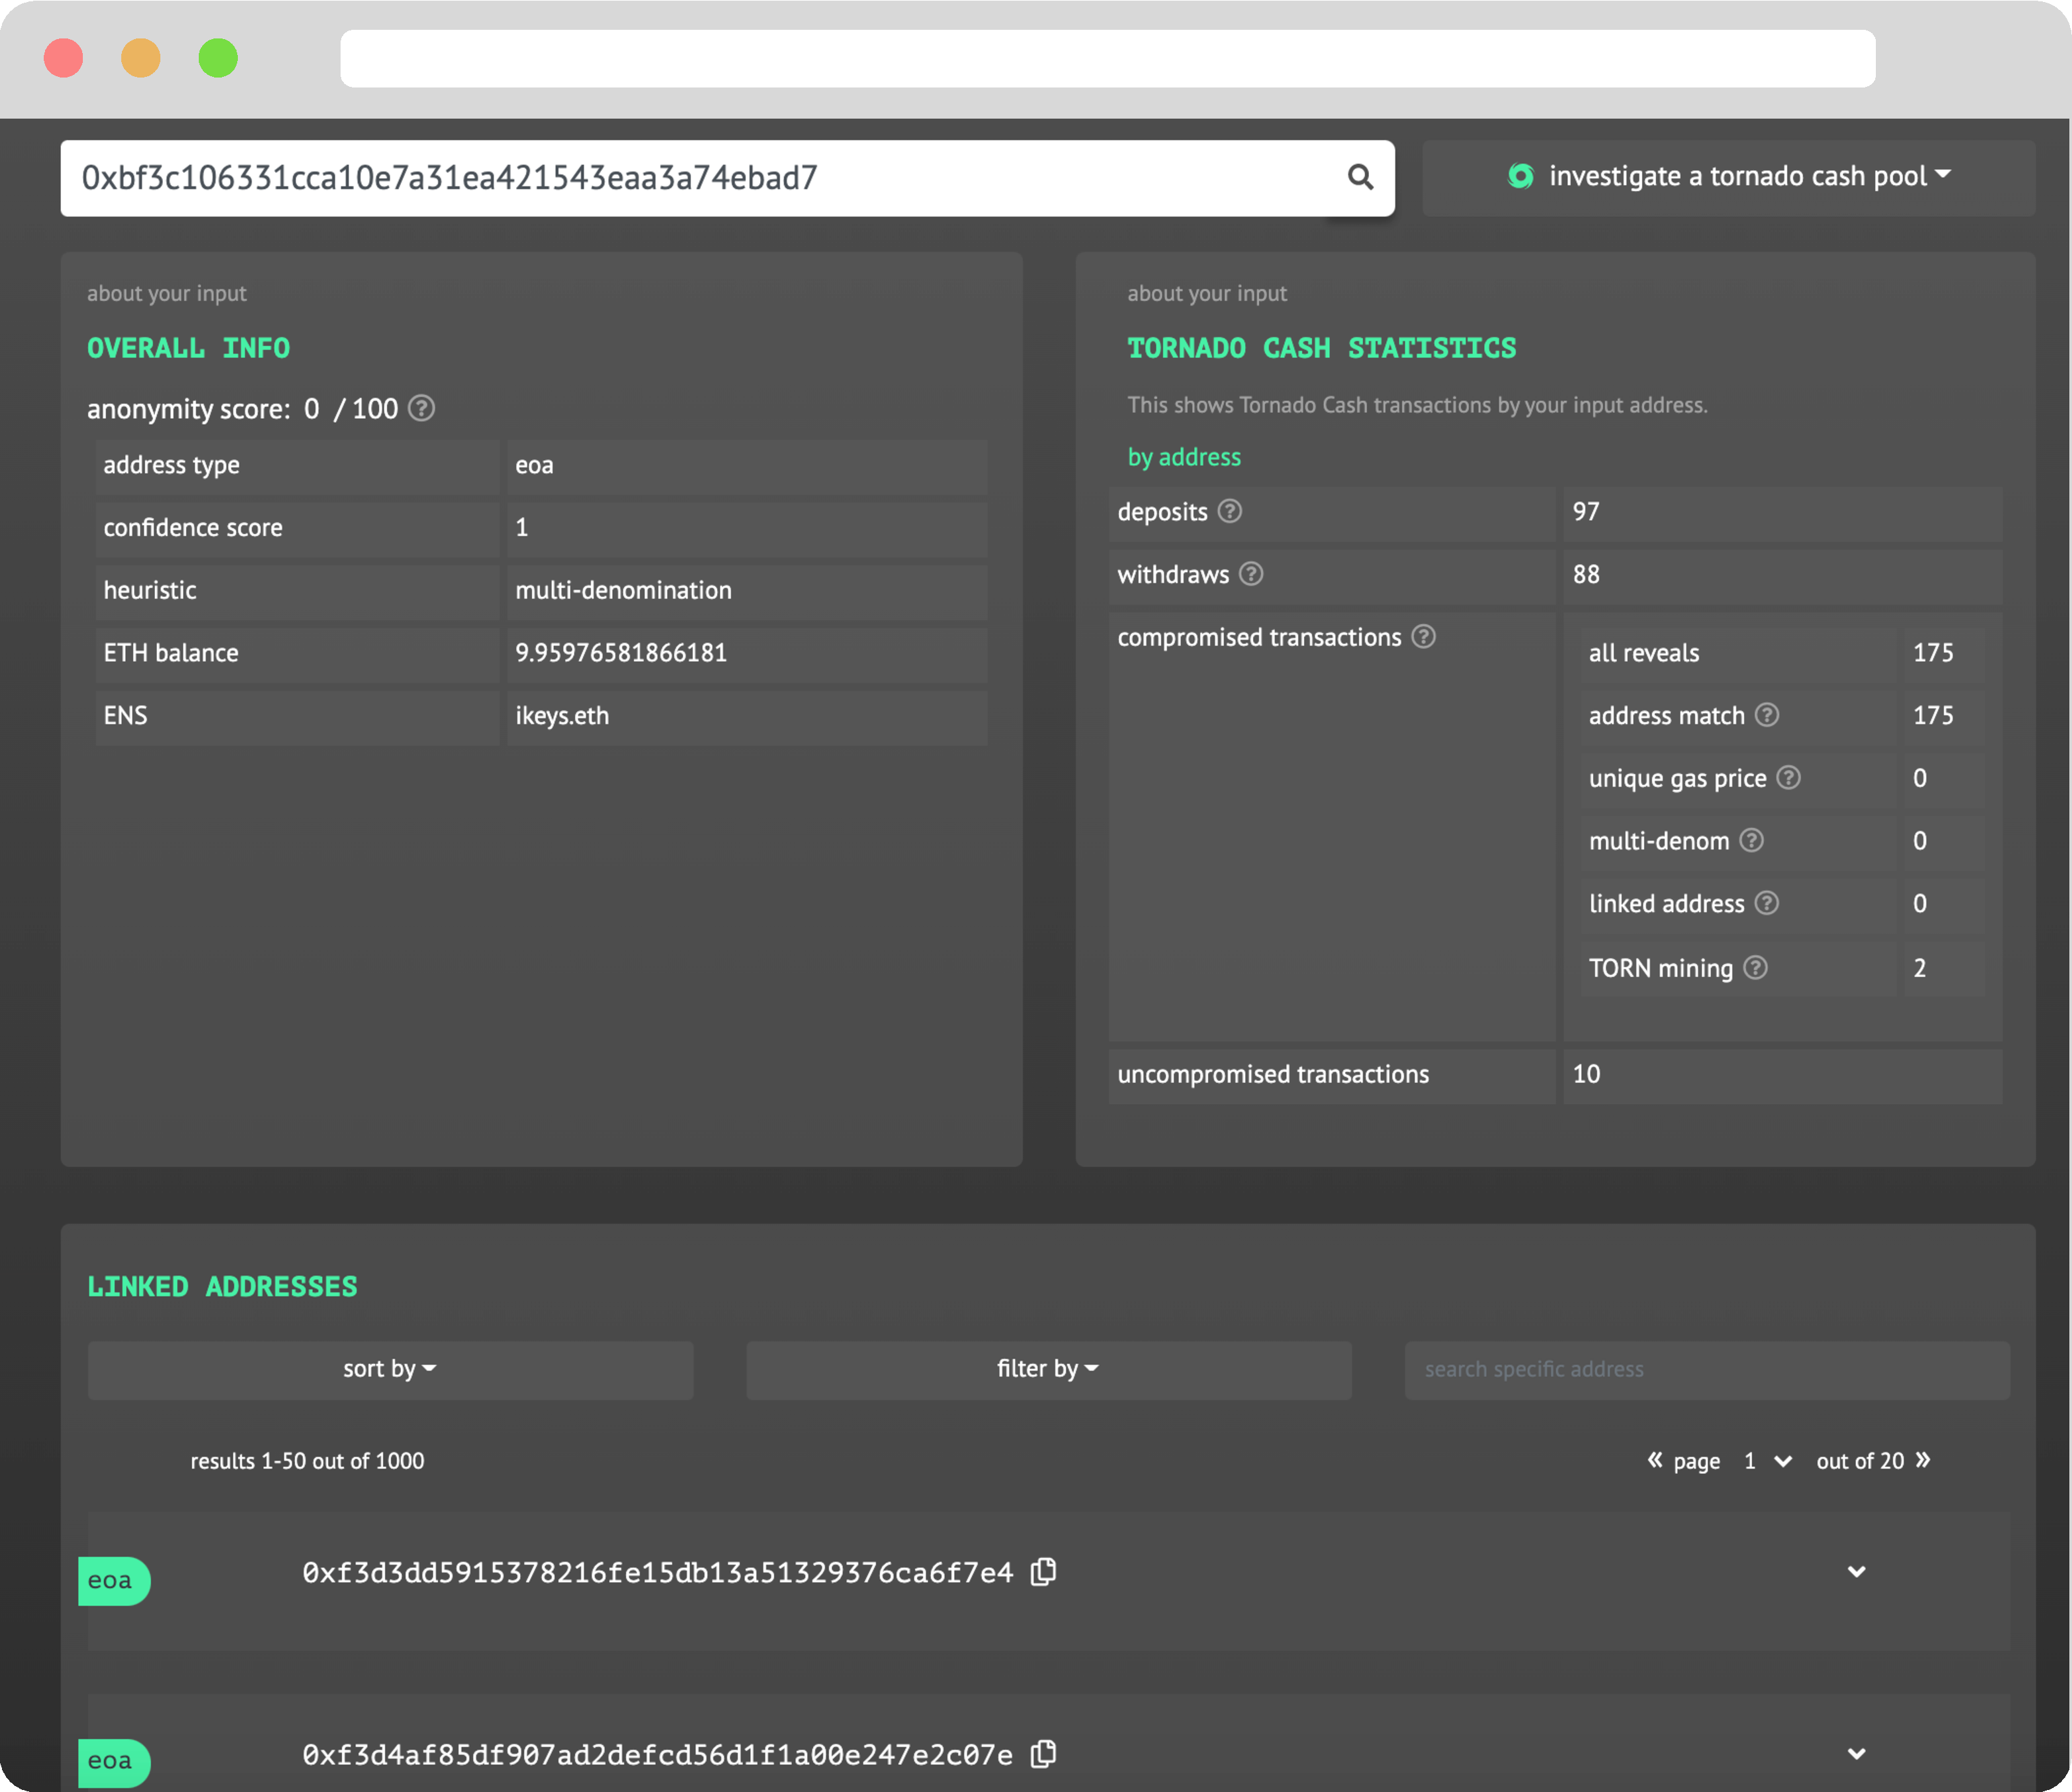
\includegraphics[width=\linewidth]{figures/demo.pdf}
\caption{Tutela interface when searching an Ethereum address. This address is also a Tornado Cash user.}
\label{fig:demo}
\end{figure}

We summarize the main functionalities shown in Figure~\ref{fig:demo}. The response page is separated into three sections. The top left section summarizes the anonymity for the searched address. It contains an ``anonymity score'' out of 100, where a lower number represents less anonymity. In this example, the searched address has an anonymity score of 0, representing a large of amount of leaked identity information. Other information, such as balance in ETH or ENS names are shown when relevant.

The top right section is only populated if the searched address is a Tornado Cash user. In this example, the searched addresses has deposited 97 times to a Tornado Cash pool while having withdrawn 88 times. Interestingly, we find that through heuristics, we are able to tie 87 of those withdraw transactions to deposit transactions, thereby meaningfully reducing the useful size of the Tornado Cash pool. See Section~\ref{sec:tornado} for more details.

Finally, the bottom section labeled ``Linked Addresses'' shows a list of addresses clustered with the searched one. Each item in this list is denoted as either an externally owned address (EOA), a deposit address, or an exchange address. Each item also contains a confidence score denoting the strength of association with the searched address, and the heuristic that bound it to the searched address.
This example shows a thousand clustered addresses, representing an entity with a large wallet portfolio (e.g. bot) -- hence why the anonymity score is zero.

\begin{figure}[h!]
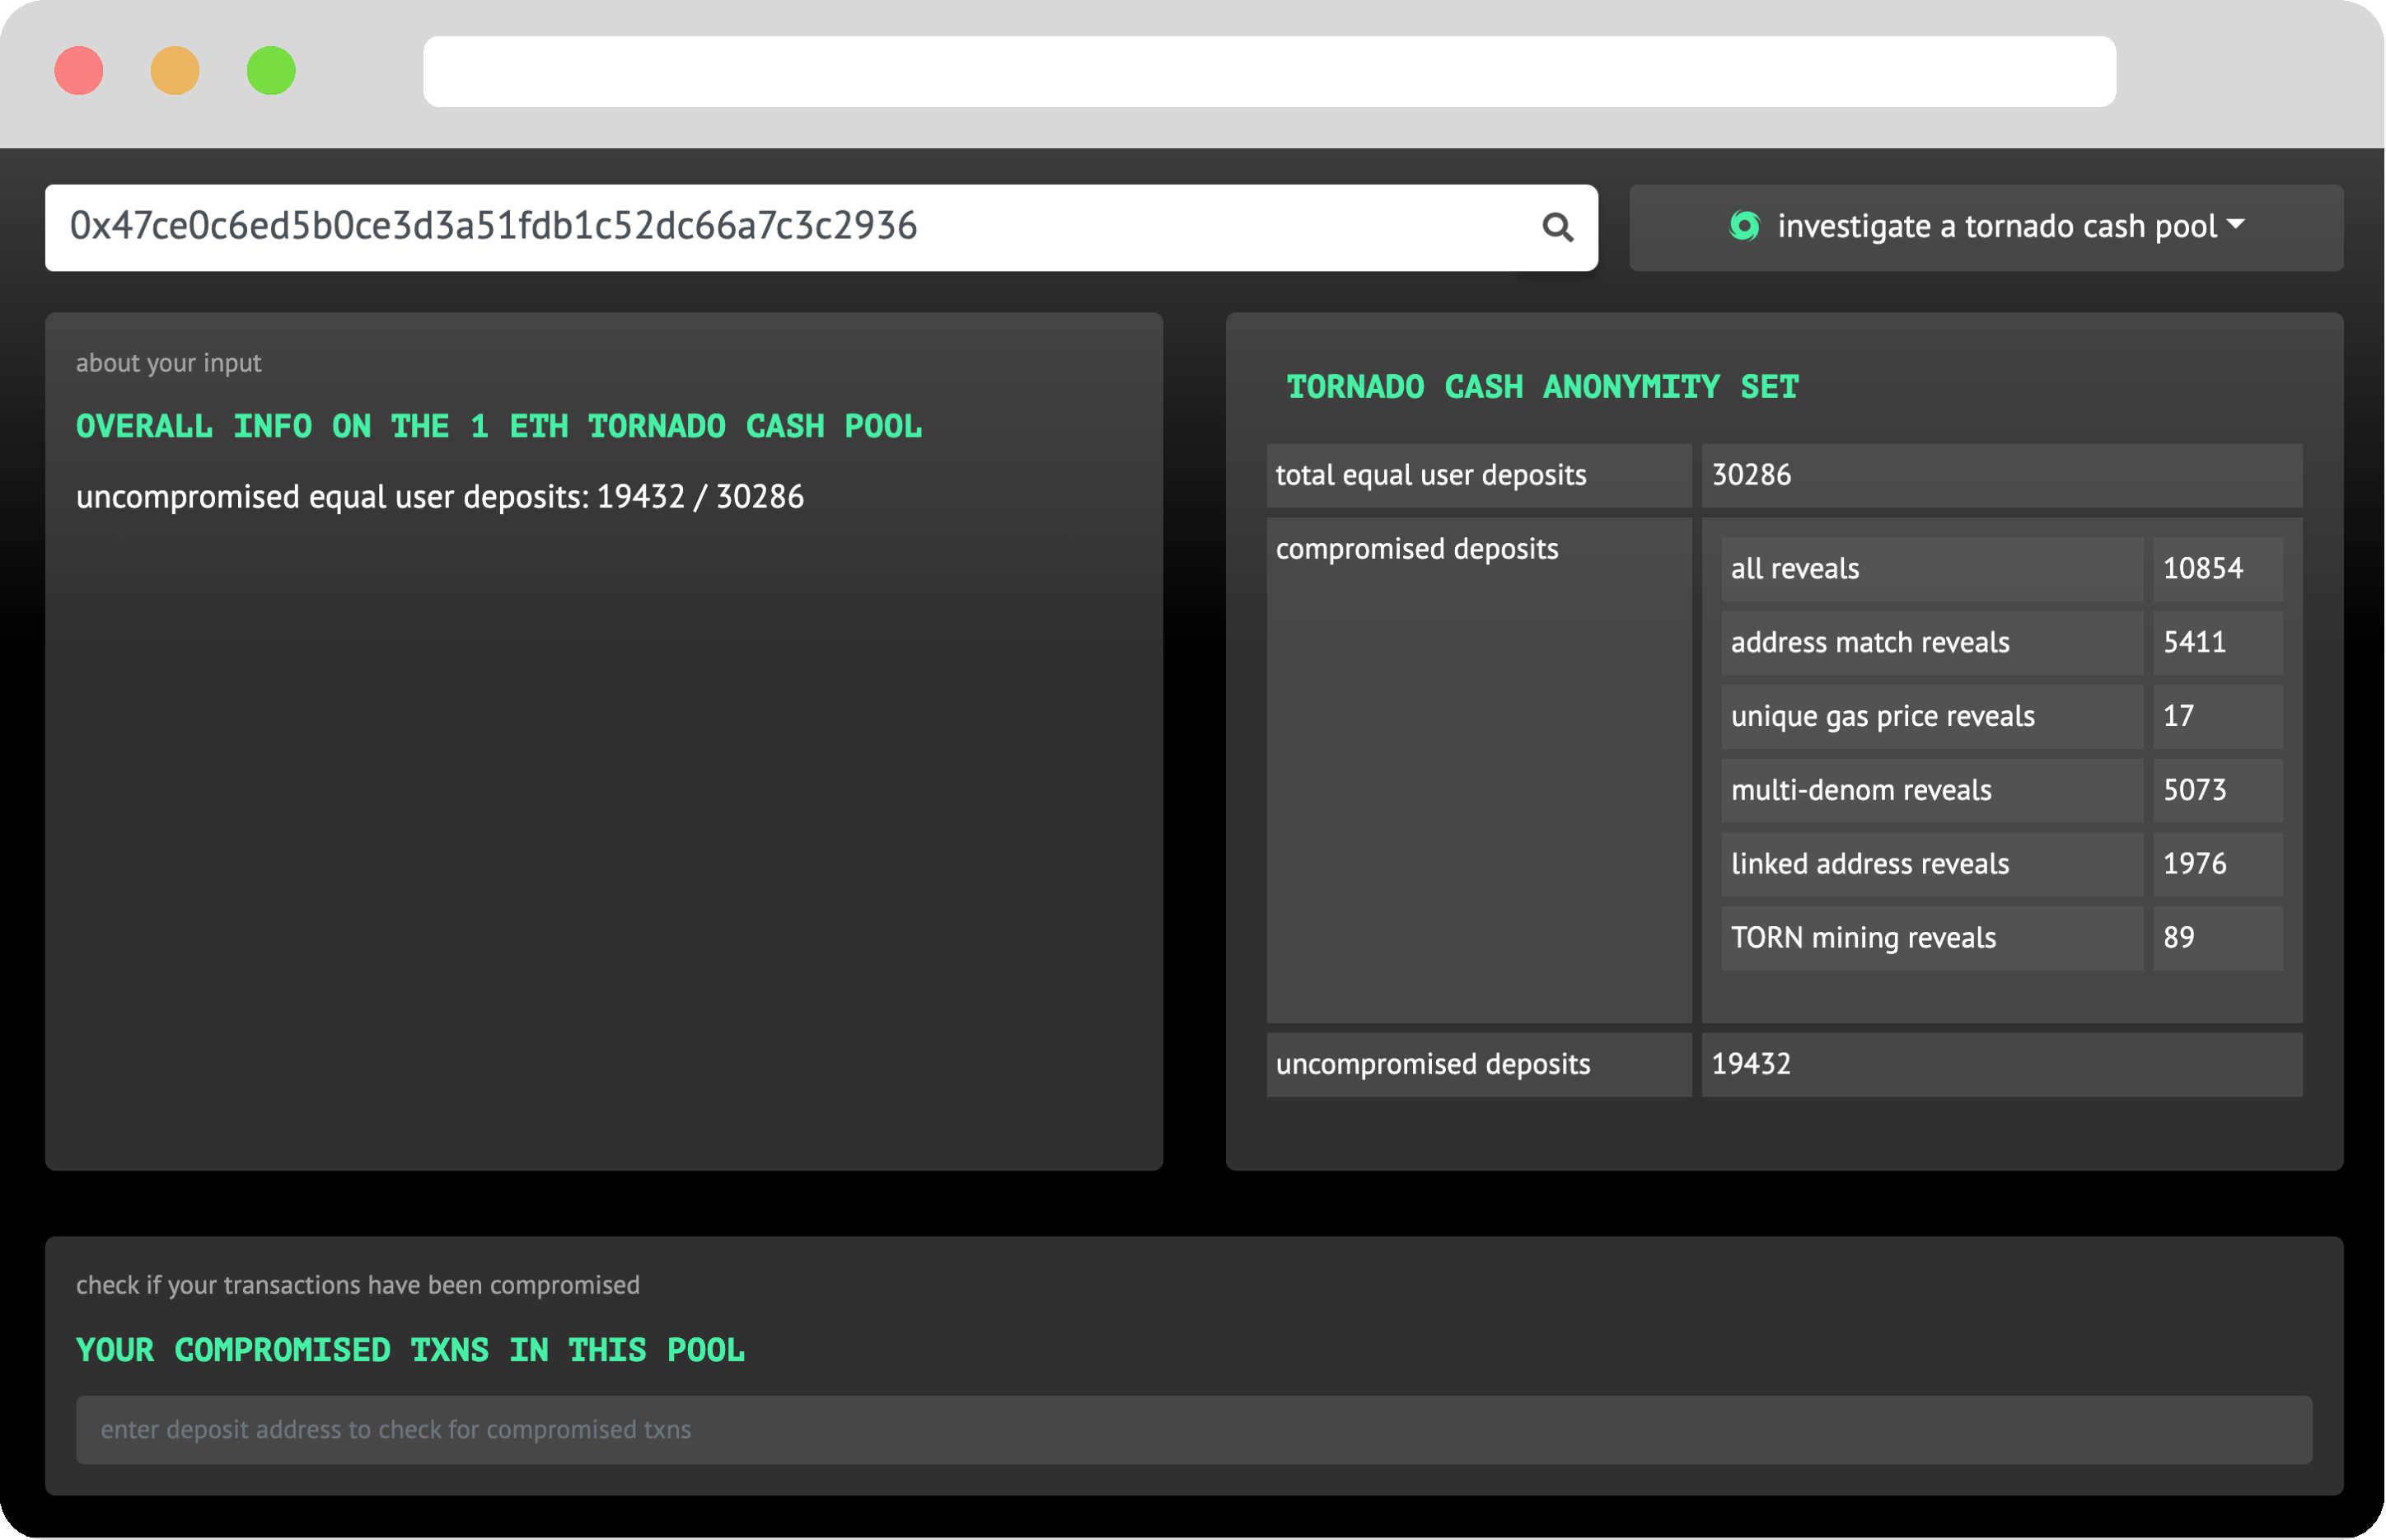
\includegraphics[width=\linewidth]{figures/demo2.pdf}
\caption{Tutela interface when searching an address corresponding to a Tornado Cash pool.}
\label{fig:demo2}
\end{figure}

If the user searches an address corresponding to a Tornado Cash pool, Tutela returns a different functionality, shown in Figure~\ref{fig:demo2}. Namely, we compute the ``true'' anonymity set size for the pool, subtracting out all equal user deposits that may have compromised through our heuristics. At the time of publication, the Tornado Cash website reports only the full anonymity set size, not taking into account potential compromises. A concrete use case of Tutela is to adjust this number to more faithfully protect the privacy of Tornado Cash users.

\section{Data and Setup}

Ethereum transactions are downloaded from the \texttt{crypto\_ethereum} dataset using BigQuery, including all transactions from August 7th, 2015 to October 1st, 2021.  In total, this amounts to 4 terbytes of data with over 1B rows.
In addition, we assume access to a list of known addresses, obtained from a public Kaggle challenge\footnote{See list of labelled Ethereum addresses found at \url{https://www.kaggle.com/hamishhall/labelled-ethereum-addresses}.}, containing almost 20,000 labelled addresses corresponding to different centralized exchanges, decentralized exchanges, relayers, DeFi applications, and more.
This list will be used to identify exchange addresses for heuristics and apply known constraints on the identity of clustered addresses.

Additionally, we create a partition of the transaction data from \texttt{crypto\_ethereum} pertaining to Tornado Cash pools. This is done by checking that the address receiving a transaction is a Tornado Cash smart contract (taken from a BigQuery dataset \texttt{tornado\_cash\_transactions}). To capture the transactions executed by the Ethereum virtual machine (e.g. through a smart contract), we use the \texttt{crypto\_ethereum.traces} table. In the special case that a withdrawal from a Tornado Cash pool is made by a relayer, we decode the input code using the contract ABI to find the recipient address. In total, we uncover around 97,365 deposit and 83,782 withdraw transactions across currency pools. These two datasets will be used for Tornado Cash -specific heuristics.

\section{Ethereum Heuristics}

Using this large dataset, we describe two Ethereum-wide heuristics used to cluster together addresses potentially belonging to the same entity.
 % After summarizing each algorithm, we will present key advantages and drawbacks.

\subsection{Deposit Address Reuse}
\label{sec:dar}

Deposit address reuse (DAR) links together EOAs through usage a centralized exchange (CEX). We refer to the original paper \citep{victor2020address} for a detailed description but provide an overview here.

\begin{figure}[b!]
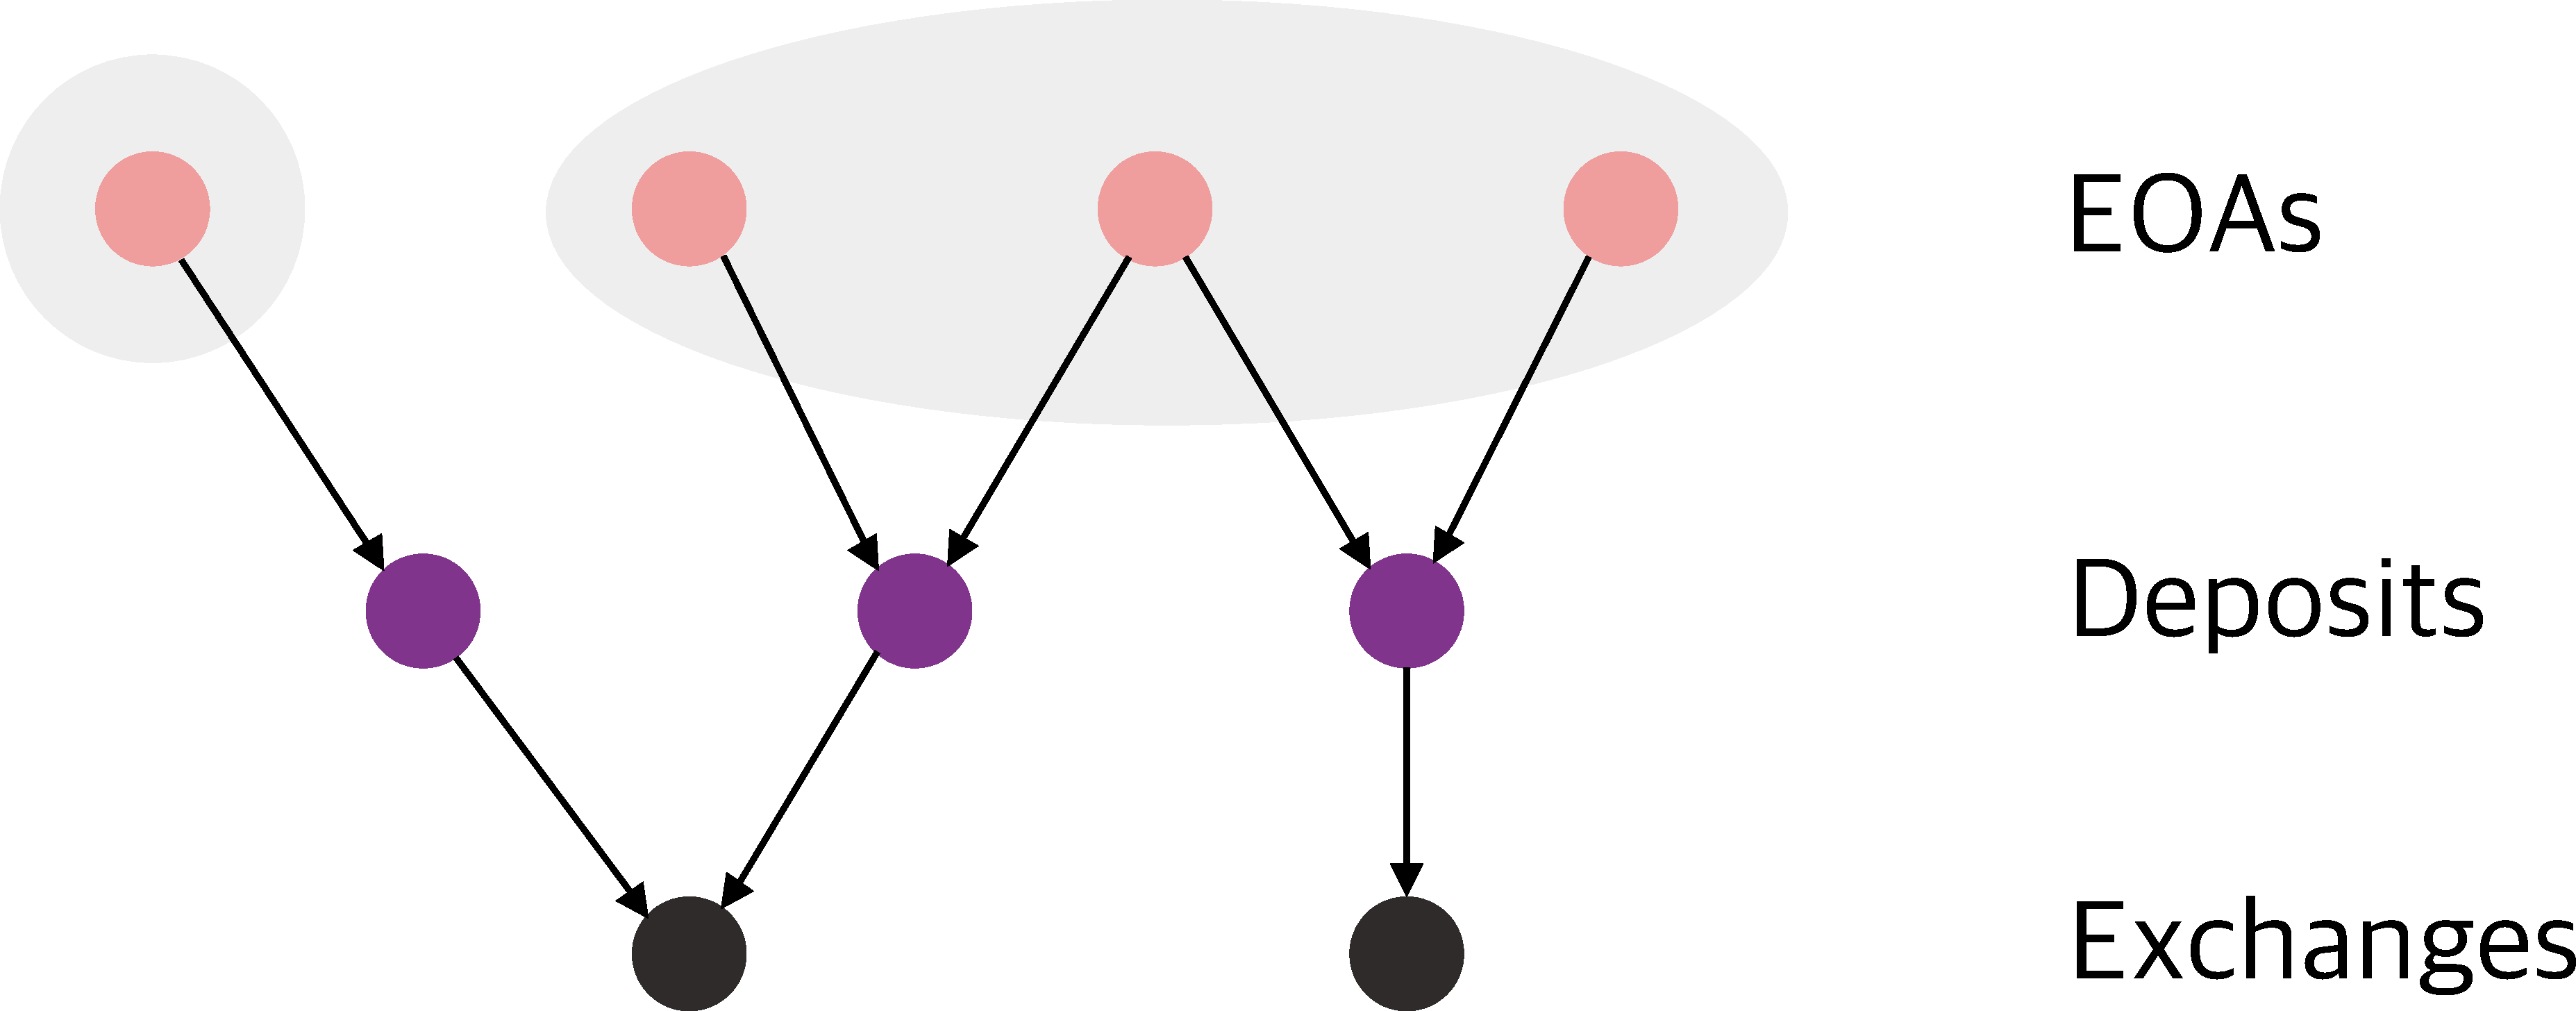
\includegraphics[width=\linewidth]{figures/dar.pdf}
\caption{Graph of transactions between EOA, deposit, and CEX addresses. A cluster is defined as a weakly connected component in an undirected subgraph containing only EOA and deposit nodes. The gray circles show EOA addresses in two clusters.}
\label{fig:dar}
\end{figure}

When users sell Ether to a CEX, the exchange typically creates ``deposit addresses'', which receive the assets from the EOA and then forward these funds to a main address associated with the CEX. Critically, these deposit addresses are created per customer, not per address. That is, multiple addresses that send funds to the same deposit address are highly likely to be owned by the same entity. However, these deposit addresses not known. The DAR algorithm seeks to identify deposit addresses through heuristics.
It uses two hyperparameters: the maximum amount difference $\alpha$ and the maximum time difference $\tau$ between two transactions: a ``receiving'' transaction from an EOA to a suspected deposit address, and a ``forwarding'' transaction from a deposit to a main exchange address (we assume access to a list of main CEX addresses). The intution is that true deposits likely forward funds quickly, and differences in amount should be only be due to transaction fees. We exclude suspected deposit addresses that are known entities (e.g. CEX, DEX, miner, etc.).

Then, we can search for $($EOA, deposit, exchange$)$ tuples that match the constraints set by $\alpha$ and $\tau$.
If we construct an undirected graph with addresses as nodes and edges between associated EOA and deposits, a ``cluster'' is defined as a weakly connected component. This definition captures interesting cases where a single entity has multiple EOAs that send to different deposits of multiple CEXs (see Figure~\ref{fig:dar}). In practice, we pick $\alpha = 0.01$ and $\tau = 3,200$ \citep{victor2020address}.

For each cluster, we would like to assign a confidence score, representing our belief in this cluster representing a single entity. We note that any uncertainty in clustering must come from uncertainty in defining deposit addresses. So, for any address in a cluster $C$, we assign  confidence as the average confidence for deposits in $C$. Now, for any deposit $v$, we define confidence as:
\begin{equation*}
\kappa(v) = 1 - \left\{ \frac{1}{2}\left(\frac{|a_f - a_r|}{\alpha}\right) + \frac{1}{2}\left(\frac{t_f - t_r}{\tau}\right) \right\}
\end{equation*}
where $a_f$ and $a_r$ are the amounts from the forwarding and receiving transactions, respectively. Similarly, $t_f$ and $t_r$ are the forwarding and receiving block numbers.
A larger difference in either amount or time would decrease the confidence, which is bound to be between 0 and 1.

\subsection{Learned Node Embedding}

The benefit of DAR is interpretability: we can understand why the algorithm believes two addresses are linked. However, this comes at the cost of recall. DAR searches for a very specific behavior, and most addresses will not be in a cluster of greater than size 1. Initial feedback from Tutela users reported limited success in finding clusters.
To supplement DAR, we consider a second Ethereum-wide heuristic that projects addresses to points in a low-dimensional vector space based on who it transacts with. In this vector space, addresses belonging to the same entity should be close together in Euclidean distance.

Consider constructing an undirected graph $G(V, E)$ from all Ethereum transactions, where nodes $V$ are composed of distinct addresses and an edge is placed between two nodes if there is a transaction between this. Each edge is given a weight $w: V \times V \rightarrow \mathbb{N}$ designating the number of interactions between two addresses. For instance, and if Alice has sent Bob 1 ETH five times,  then $w(\textup{Alice}, \textup{Bob}) = 5$. Note that this graph is distinct from the one used in Section~\ref{sec:dar}.

At this abstraction layer, we seek to learn a ``node embedding function'' $f: V \rightarrow \mathbb{R}^d$ that projects a node to a $d$-dimensional vector representation. Importantly, we want this embedding to capture semantic information about the node, such as which other addresses it frequently interacts with. To do so, we leverage popular graph representation learning algorithms \citep{grover2016node2vec,rozemberczki2018fast}. In particular, we focus on Diff2Vec \citep{rozemberczki2018fast}, which has been applied to blockchain transactions \citep{beres2021blockchain}, though not at scale.

The intuition of Diff2Vec is to summarize a node by its neighborhood through a diffusion-like random process. Specifically, there are four steps to Diff2Vec: (1) generating a ``diffusion graph'', (2) sampling a ``node sequence'', (3) extracting features, (4) learning a neural network embedding. We briefly summarize each step below.

\paragraph{Step One} Fixing a starting node $v \in V$, we initialize a diffusion subgraph $\tilde{G}$ containing only $\{v\}$. Then, we randomly sample a node $u$ from $\tilde{G}$, then randomly pick $w \in \textup{Neighors}(u, G)$, where $G$ is the original graph. Add node $w$ and the edge $(u, w)$ to $\tilde{G}$. Repeat until $\tilde{G}$ has $l$ nodes, where $l$ is a hyperparameter representing the amount of information we want to capture in our eventual node embedding. A larger $L$ may capture a large neighborhood but sacrifice in granularity.

\paragraph{Step Two} Given $\tilde{G}$, we generate a sequence $s = (v_1, v_2, \ldots)$ recording the notes visited during an Euler walk. To do this, we must ensure that $\tilde{G}$ is Eulerian, which holds if every node has an even degree. A simple way to achieve this is to double each edge in $\tilde{G}$. At this point, we can summarize a node $v \in V$ by multiple sequences $S = (s_1, s_2, \ldots)$, each from a random walk.

\paragraph{Step Three} Given a set of sequences $S$, we aim to produce a single feature vector based on frequencies of which vertices appear near each other in sequences $s \in S$. Specifically, fix a node $v$. Then, pick a window size $h$.
Count how many times other nodes appear within $h$ positions before and after when $v$ appears, summed over all sequences $s \in S$. This will result in $2h$ vectors each of length $|V|$ --- $2$ from counting before \textit{and} after; $h$ from counting frequences 1 to $h$ positions away from $v$; $|V|$ since each vector stores counts of all nodes in $V$. Denote this feature vector by $y(v) \in \mathbb{R}^{2h|V|}$.

\paragraph{Step Four} Finally, we wish to compress the feature vector from Step Three to a $d$-dimensional continuous space. To do this, we train a two layer perceptron $f_\theta = f_1 \circ f_2$ using stochastic gradient descent \citep{goodfellow2016deep,kingma2014adam}. Define $f_1: \mathbb{R}^{|V|} \rightarrow \mathbb{R}^d$ and $f_2 \mathbb{R}^d \rightarrow \mathbb{R}^{2h|V|}$, with a ReLU nonlinearity in between. The input to the network is a one hotted representation of the current node $v$.
To train the parameters $\theta$, we optimize the objective
\begin{equation}
  \mathcal{L}(v; \theta) = \texttt{dist}(f_\theta(\texttt{one\_hot}(v)), y(v))
  \label{eq:obj}
\end{equation}
where $\texttt{dist}$ is a distance function. Example include Euclidean distance, or a cross entropy loss.
That is, Equation~\ref{eq:obj} optimizes $f_\theta$ to predict the frequency vector. Then, assign $f_1(v) \in \mathbb{R}^d$ to be the final embedding for $v$.\newline

Steps three and four amount to Word2Vec\footnote{We use \texttt{gensim.models.word2vec}.} \citep{mikolov2013efficient,mikolov2013distributed}. In practice we optimize with SGD for 10 epochs with a learning rate of 0.05. We set $d = 128$, $l = 80$, and $h = 10$. Given an address $v \in V$, to find its cluster, we can search for the closest $k$ vectors in $\mathbb{R}^d$. Unlike DAR, this heuristic will always return $k$ addresses. We score the confidence of an address $u$ in the cluster by its Euclidean distance to the embedding of $v$:
\begin{equation*}
\kappa(u) = \frac{1}{\|f_\theta(\texttt{one\_hot}(u)) - f_\theta(\texttt{one\_hot}(v))\|_2}
\end{equation*}
since a smaller distance (closer to 0) represents more semantic similarity or $u$ to $v$.

\subsection{Anonymity Score}
\label{sec:anonymityscore}

\section{Tornado Cash Heuristics}
\label{sec:tornado}

\subsection{Address Match}

\subsection{Unique Gas Price}

\subsection{Multiple Denomination}

\subsection{Interaction History}

\section{Analysis}

TODO. This is where most of the heavy lifting needs to happen.

\section{Discussion and Future Work}

\subsection{Limitations}



\subsection{Extensions}

offchain data

\subsection{Broader Impact}

chainanalysis, regulation (@will)

\section*{Acknowledgments}
We would like to acknowledge both the Tornado Cash team and the Convex Research team for their support. This work was funded by the Tornado Cash community bounty to develop anonymity tools to protect user privacy. We also thank the Tornado Cash community at large for their consistent feedback and patience through our application's development. Finally, we thank the Stanford Venture Studio for their support with compute credits.

\bibliography{whitepaper}
\bibliographystyle{acl_natbib}

\end{document}
